\documentclass[10pt]{report}
\usepackage[utf8]{inputenc}
\usepackage[top=2cm, bottom=2cm, left=2cm, right=2cm]{geometry}
\usepackage[francais]{babel}
\usepackage{helvet}
\usepackage[T1]{fontenc}
\usepackage{graphicx}
\usepackage{subcaption}
\usepackage{etoolbox}
\renewcommand{\familydefault}{\sfdefault}

% Supprime l'espace avant l'en-tête des chapitres
	\makeatletter
	% les chapitres normaux
	\patchcmd{\@makechapterhead}{\vspace*{50\p@}}{}{}{}	
	% les chapitres étoilés
	\patchcmd{\@makeschapterhead}{\vspace*{50\p@}}{}{}{}
	\makeatother

\begin{document}

\begin{titlepage}	
	\flushleft
	\begin{figure}[!h]
		\includegraphics[height=1.8cm]{Reports/figures/logo_insa_cvl.png}
		\hfill
		\includegraphics[height=3cm]{Reports/figures/logo_biomedia.png}
	\end{figure}
	\centering
	\vspace{2cm}
	{\scshape\Large Stage industriel de 4ème année\par}
	\vspace{1.5cm}
	{\huge\bfseries Développement d'une bibliothèque mathématique performante pour le traitement d'images médicales\par}
	\vspace{2cm}
	{\Large\itshape Élève ingénieur: François PIAT\par}
		\vspace{1cm}
	\begin{figure}[!h]
		\begin{center}
			\includegraphics[width=13cm]{Reports/figures/biomedia_image.png}
		\end{center}
	\end{figure}
	\vfill
	\flushleft
	Tuteur INSA: \hfill Tuteur BioMedIA: \par
	Julien \textsc{Olivier} \hfill Ghislain-Anthony \textsc{Vaillant}
	\vfill
	% Bottom of the page
	\centering
	{\large Année universitaire 2015 - 2016 \par}
\end{titlepage}

\section*{Remerciements}\newpage
\paragraph*{Résumé} % dans cet ordre
\paragraph*{Mots-clés}
\paragraph*{Abstract}
\paragraph*{Key-words}

% sommaire
\renewcommand\contentsname{Sommaire}
\tableofcontents

\newpage

\chapter*{Introduction}
\addcontentsline{toc}{chapter}{Introduction}
\chapter{Environnement de travail} 
	\section{Le laboratoire}
		Le laboratoire BioMedIAest implanté sur le campus principal de l'Imperial College London, dans le quartier du South Kensington. Il fait partie du groupe de recherche en traitement visuel d'informations (Visual Information Processing) au sein du département informatique de l'université.
	\subsection{Imperial College London - Department of computing}
%	Domaine d'activité, stats, organigramme

	
	%	Visual Information Processing research covers a range of topics including vision, graphics, intelligent behaviour understanding, and biomedical image computing.
	%	
	%	The work of the section has led to more than 8 best paper awards at major international conferences (IEEE FG, ICRA, ISMAR, MICCAI, SensorComm) and attracted four Marie Curie fellows.
	%	
	%	The group has pursued a successful strategy of growth in several key areas:  novel modelling and filtering approaches for SLAM and real-time dense scene mapping.
	%	
	%	Intelligent behavior understanding, novel approaches to facial action and emotion prediction as well as novel approaches to robust face alignment, tracking and expression recognition, biomedical imaging computing, robotics & sensing, and appearance modelling for realistic computer graphics.
	\paragraph{Imperial College London}
		\begin{figure}[h!]
			\begin{center}
				\includegraphics[width=16cm]{Reports/figures/College-Organisation.pdf}
			\end{center}	
			\caption{Organigramme de l'Imperial College London}
			\label{Organigramme de l'Imperial College London}
		\end{figure}
	La recherche en traitement visuel d'informations intervient dans de nombreux domaines tels que la visualisation, le graphisme, la compréhension intelligente, et le traitement d'images biomédicales.  
	Les travaux du département ont été récompensés de 8 titres lors de conférences internationales majeures (IEEE FG, ICRA, ISMAR, MICCAI, SensorComm) et de 4 prix Marie Curie.
	

	
	\subsection{BioMedIA}
%	Synopsis, détail des activités du laboratoire
	
	La mission du groupe BioMedIA est de développer de nouvelles techniques de
	calcul pour l'analyse d'images biomédicales. Le groupe se concentre sur des
	domaines de recherche de pointe, y compris:\\

	{$\bullet$} Le développement d'algorithmes d'acquisition, d'analyse et d'interprétation
	des images. En particulier dans les domaines du recalage, de la reconstruction,
	du suivi de mouvement, de la segmentation et de la modélisation. \\

	{$\bullet$} L'apprentissage machine pour l'extraction d'information clinique à partir
	d'images médicales. Les applications incluent le diagnostic assisté par
	ordinateur, la planification automatisée de traitement médicale, ou encore les
	interventions et la thérapie guidées par ordinateur. \\

	Nous nous intéressons particulièrement à l'imagerie et les technologies de
	traitement informatique qui nous permettent de mieux comprendre le
	développement du cerveau humain, l’évolution des maladies mentales et le
	diagnostic des patients atteints de maladie cardiovasculaire.
	
	
	\section{Cadre du projet} % présentation de MIRTK, de ses applications, de son architecture(modules, fonctions...).
	\paragraph{Le logiciel étudié}~\par~\par
	Medical Image Registration Tool-Kit (abrégé MIRTK) est un logiciel open-source de traitement d'image médicales utilisé par des chercheurs dans le milieu médical. Le cahier des charges provient majoritairement de ces chercheurs, qui ont des besoins variables en termes de visualisation. Le logiciel est adapté en conséquence par la suite. Par conséquent, MIRTK, qui est codé en C++, comporte un nombre important de classes et de fonctions diverses, destinées à couvrir le maximum des besoins des chercheurs.
	Afin de rester pertinent pour ces chercheurs, MIRTK nécessite donc une maintenance et une amélioration continue. 

	 % - logiciel de traitement d'image médicales, utilisé par les chercheurs en milieu médical.
	 % - stable mais nécessite une maintenance et une amélioration continue pour rester pertinent.
	 % - Intervention sur le module "Numerics", bibliothèque mathématique.
	 \paragraph{UK BioBank}~\par~\par
	  A long terme, MIRTK serait potentiellement destiné a faire partie d'un projet global pour la UK BioBank qui prévoit de regrouper la plus grosse banque de données médicales, incluant notamment des données visualisables. Cette base de données regroupera aussi des dizaines de caractéristiques pour chaque patient (habitude alimentaires, antécédents médicaux, génotype...). Afin de pouvoir traiter un tel nombre de données, MIRTK n'est pas suffisamment optimisé. Le but principal de ce stage est donc de commencer la démarche d'amélioration du logiciel en terme de design et de performances.
	 

\chapter{Objectifs et cahiers des charges}
	\section{Problématique} %Inclure contexte du projet, avec la raison pour laquelle ce projet est nécessaire.
	%(back-end math) dépendances externes : eigen et boost + noyaux internes implémentés via TBB => inconsistence => parrallélisation existante floue , efficacité = ? performances=? => profilage	===> n'utiliser qu'une seule dépendance (externe) : ArrayFire qui peut amener l'optimisation via GPU (résumer ça en 3 points majeurs) 
	Tel que décrit dans le titre du stage, les notions abordées seront reliées, dans un premier temps aux performances de MIRTK, pour cela, M. Maxime NOEL et moi-même sommes intervenus sur différents niveaux d'abstraction du logiciel. Mon collègue s'est d'avantage concentré sur l'enchaînement des exécutions, et l'interface MIRTK/utilisateur (cf stage intitulé" \textbf{?????????????????????????????????????????}"), tandis que je suis intervenu dans les couches logicielles les plus basses, et les plus directement reliées aux composants hardware. \\
	
	La majeure partie du stage sera donc axée sur le back-end mathématique de MIRTK, c'est-à-dire les fonctions appliquant des opérations matricielles sur les images d'entrée par exemple. L'un des problèmes majeurs de MIRTK est sa forte dépendance de plusieurs bibliothèque qui, chacune, ne sont pas utilisées au maximum de leur potentiel, il s'agit de EIGEN, BOOST et TBB, dont les rôles sont définis ci-dessous:\\
		\\{$\bullet$} \textit{EIGEN:} cette bibliothèque fournit les fonctions essentielles en termes de manipulation de matrice. \newline
		\\{$\bullet$} \textit{BOOST:} écrite en C++, cette bibliothèque fournit des outils d'algèbre linéaire, de traitement d'image ou encore de génération de nombres pseudo-aléatoire... \newline
		\\{$\bullet$} \textit{Threading Building Blocks (TBB)}: TBB permet l'implémentation de boucles a exécuter en parallèle. L'exécution parallèle (ou \textit{multi-threading}) est une méthode d'optimisation des performances d'un logiciel. Elle consiste a dédier plusieurs "threads" à son exécution, et transforme donc un processus itératif tel qu'une boucle FOR en une répartition de toutes les itérations, mais exécutées en simultanées. Le temps d'exécution est donc au final considérablement réduit. \newline
	\\ Ainsi, l'inconsistance de MIRTK autour de ces 3 bibliothèques implique des performances parfois médiocres, et surtout une parallélisation réalisée de manière assez floue, dont l'efficacité est encore à prouver.  
	\\ C'est pour cette raison, que l'apport d'une bibliothèque coordonnant des fonctions issues d'au moins 2 des 3 dépendances précédentes sera un véritable avantage si les performances du logiciel sont améliorées, ou même si elles demeurent inchangées. 
		

	 

	\section{Cahier des charges}
%	Lister les attentes et les contraintes du projet.
	ArrayFire pourrait être la bibliothèque la plus adaptée pour ce genre de situation puisqu'elle est similaire à l'actuelle bibliothèque EIGEN, mais en permettant l'optimisation du logiciel. Pour palier cette faiblesse d'EIGEN, TBB était nécessaire, mais pas avec ArrayFire. De plus, ArrayFire ajoute la possibilité de gérer le changement de back-end afin de travailler sur un GPU (carte graphique), ou sur un CPU (processeur).\\
	\\
	Avec cette bibliothèque, il va être possible de réaliser les points suivants:\\ 
		\\{$\bullet$} Revoir les fonctions les plus coûteuses en ressources et dont les performances sont les plus médiocre, en les recodant avec ArrayFire.\\
		\\{$\bullet$} Supprimer intégralement toute dépendance à TBB puisque la parallélisation du code se fera exclusivement avec ArrayFire.\\
		\\{$\bullet$} La programmation sera réalisée de manière transparente, c'est-à-dire que MIRTK doit réaliser les mêmes fonctions et garder le même front-end même si le code plus en profondeur est modifié. En revanche, il sera possible d'ajouter des options d'exécution, notamment en ce qui concerne la gestion des back-end.\\
		\\{$\bullet$} Plusieurs benchmarks devront affirmer la pertinence du nouveau code de MIRTK en comparant les test de performances avant et après l'intégration d'ArrayFire.\\
%(Le délivrable sera composé IDEALEMENT de 2 backends, l'un AF et l'autre EIGEN. En fonction des applications, un switch automatique entre chaque structure sera appelé en dur grâce à des commandes pré-proc.) => étape bonus
		\\{$\bullet$} A l'issue du stage, s'il reste suffisamment de temps pour s'y intéresser, il serait idéal d'implémenter une fonctionnalité de changement automatique de back-end en fonction des performances de EIGEN et ARRAYFIRE sur une fonction en particulier. En se basant purement sur un critère de performances, on pourrait par exemple avoir une génération de matrice initiée par EIGEN puis une rotation de matrice exécutée par ArrayFire. Les commandes de changement automatique de back-end seront idéalement codées dans le pré-processeur du code de MIRTK. Il restera tout de même une possibilité d'empêcher cette bascule automatisée (qui sera au final définie par défaut) par commande manuelle.
	\\
	\\
	\textit{Je tiens à préciser que le cahier des charges listé ci-dessus sont idéaux. Ne sachant pas à quoi s'attendre lors de l'étude de MIRTK, il se peut que ces différents points se voient modifiés, en fonction de la difficulté, du temps requis ou encore de la possibilité de leur réalisation.} 
	\section{Stratégie employée}
	\subsection{Objectifs} 
%	Détailler les objectifs a atteindre idéalement.
	- Ajouter ArrayFire à MIRTK, en remplaçant les fonctions d'EIGEN les moins adaptées par les fonctions d'AF. \newline
	- Faire un profiling des fonctions concernées par TBB, et interpréter les résultats afin d'élaborer une stratégie pour implanter la programmation // d'AF.\newline
	- Supprimer les TBB inutiles ou peu efficaces, et remplacer les autres par l'équivalent d'AF (gfor).\newline
	
	\vspace{5cm}
	\subsection{Diagramme de GANTT}
	 => gantt chart prévisionnel (à mettre en français)
	\begin{figure}[h!]
		\begin{center}
			\includegraphics[width=18cm]{Reports/figures/estimated_gantt.png}
		\end{center}	
		\caption{Diagramme de GANTT prévisionnel}
		\label{Diagramme de GANTT prévisionnel}
	\end{figure}
\chapter{Réalisation}
	\section{Profilage}
%	Définir le profilage et expliquer la nécessité d'une telle étape dans ce contexte\newline
	Lors du début de mon stage, il a fallu que je me familiarise avec les dépendances de MIRTK, mais aussi a son fonctionnement interne. C'est lors de cette étude préliminaire que mon tuteur et moi avons étudié, en plus de la bibliothèque EIGEN (destinée aux fonctionnalité mathématiques), la bibliothèque TBB, qui a pour but de mettre en place une parallélisation d'un logiciel. Constatant qu'ArrayFire était constitué de fonctions mathématiques déjà optimisées sur ce plan, il a été convenu de faire un profilage de MIRTK avant d'y intégrer ArrayFire afin de prioriser les points les plus coûteux en ressources de MIRTK. 
	\paragraph{Choix du profileur}
	Afin de discerner au mieux les performances de MIRTK, le choix du profileur (l'outil faisant le profilage) était important. Le principal poste utilisée pour le profilage travaille sur un processeur INTEL, ce qui nous a convaincu de ne pas utiliser le profileur CodeXl puisque nous avons compris après installation qu'il ne fonctionnait qu'avec des processeurs AMD. On a ensuite basculé sur VTune, développé par les collaborateurs directs d'AMD, mais nous ne l'avons pas retenu non plus de part sa complexité d'installation sur l'ordinateur souhaité.
	
	Nous avons donc finalement choisi d'utiliser l'outil Callgrind de la suite VALGRIND, capable d'analyser à la fois la quantité d'instructions envoyées au run-time, et aussi les fuites de cache.
%	=> on identifie les fonctions sur lesquelles agir en premier
	On utilise Valgrind, qui, avec callgrind analyse la manière dont les caches sont utilisés.
%	Expliquer le choix de valgrind, parmi les autres profileurs
 => projet open-source multi-plateforme et disponible dans les packages linux, autres alternatives étudiées (VTUNE intel, installation compliquée, et codeXL, qui nécessite des proc AMD).\\
	
	
	Les tests ont été effectués sur une machine dont les caractéristiques sont les suivantes : \newline
	{$\bullet$} \textit{Nombre de coeurs:} 8, 2 threads chacun\newline
	{$\bullet$} \textit{Cadence:} 1.6 GHz \newline
	{$\bullet$} \textit{Nombre de caches:} 4 \newline
	{$\bullet$} \textit{Taille des caches:}32k, 32k, 256K, 8192K \newline
	ajouter le maximum de détails (RAM, nom du proc ...)\newline
	Pour une quantité réduite de tests, et afin de cibler les modèles d'utilisation de TBB à remplacer, on a pris l'une des fonctions les plus sollicitées dans MIRTK, il s'agit d'une fonction nommée \textit{transform-image}, et qui dispose de 5 options, définissant un type d'interpolation mathématique : Linéaire (par défaut), méthode voisin le plus proche (NN), gaussienne, sinus cardinal et B-Spline. 
	
	\subsection{Analyse du nombre d'instructions}
	
	Placer ici des graphiques de performances, avec leurs interprétation
	\subsection{Analyse des fuites de cache}
	Graphique: 
		\begin{figure}[h!]
			\begin{center}
				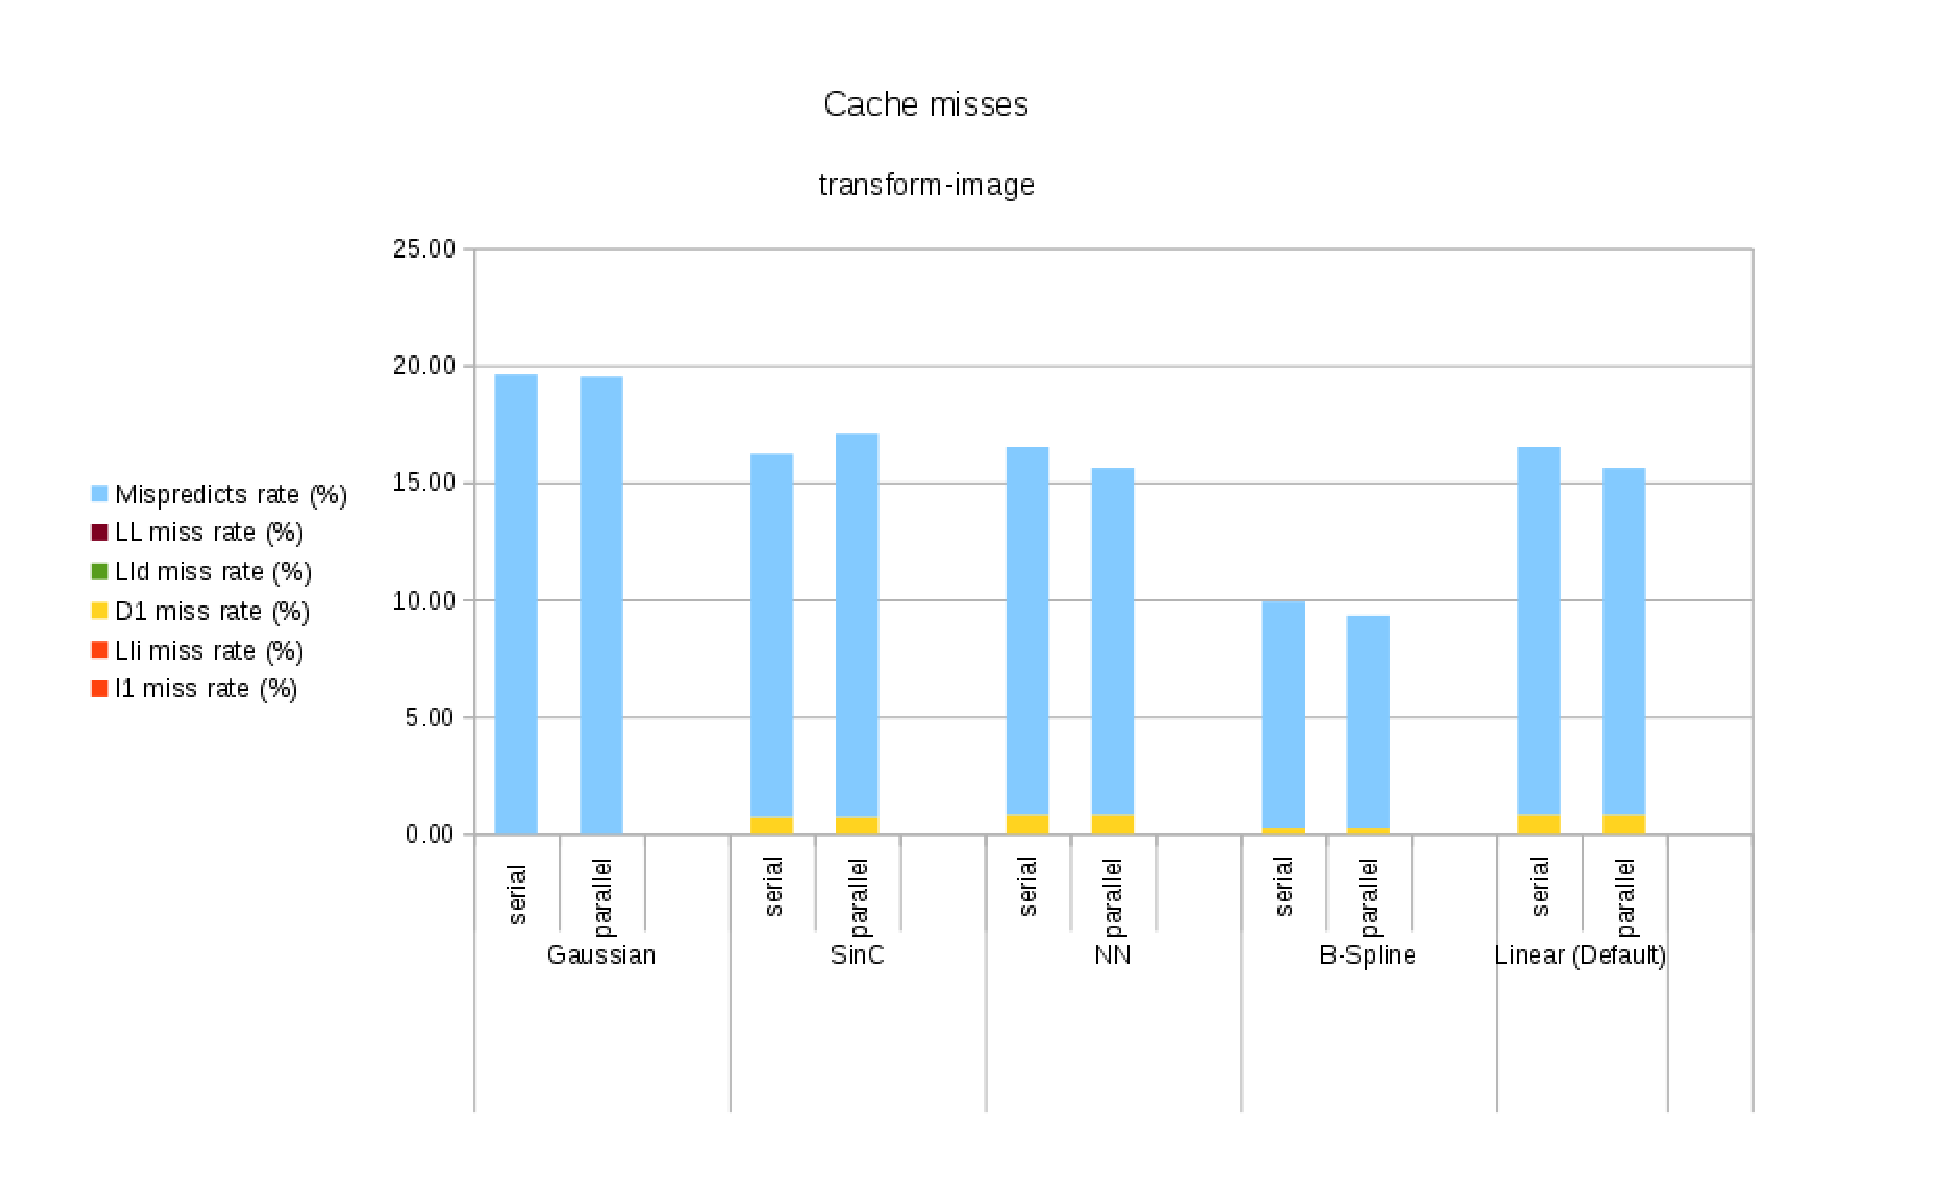
\includegraphics[width=15cm]{Reports/figures/cache_misses_transform_image.eps}
			\end{center}	
			\caption{Fuites de cache pour la fonction transform-image}
			\label{Fuites de cache pour la fonction transform-image}
		\end{figure}
	
	
	\section{Integration d'ArrayFire dans MIRTK}
	\subsection{Implémentation du module mathématique}
%	Programmation transparente entre Eigen et ArrayFire.
%	Lister les fonctions principales à substituer.
Smooth image :
	\begin{figure}[h!]
		\begin{center}
			\includegraphics[width=12cm]{Reports/figures/gaussianblurring.png}
		\end{center}	
		\caption{Algorithme de flou gaussien incluant Arrayfire - Implémentation naïve}
		\label{Algorithme de flou gaussien incluant Arrayfire - Implémentation naïve}
	\end{figure}
	\begin{figure}[h!]
		\begin{center}
			\includegraphics[width=12cm]{Reports/figures/mygaussianblurring.png}
		\end{center}	
		\caption{Algorithme de flou gaussien incluant Arrayfire - Implémentation optimisée}
		\label{Algorithme de flou gaussien incluant Arrayfire - Implémentation optimisée}
	\end{figure}
	\subsection{Gestion de la programmation parallèle}
%	Optimisation des threads et suppression de TBB au profit de ArrayFire.
Principe :
	\begin{figure}[h!]
		\begin{center}
			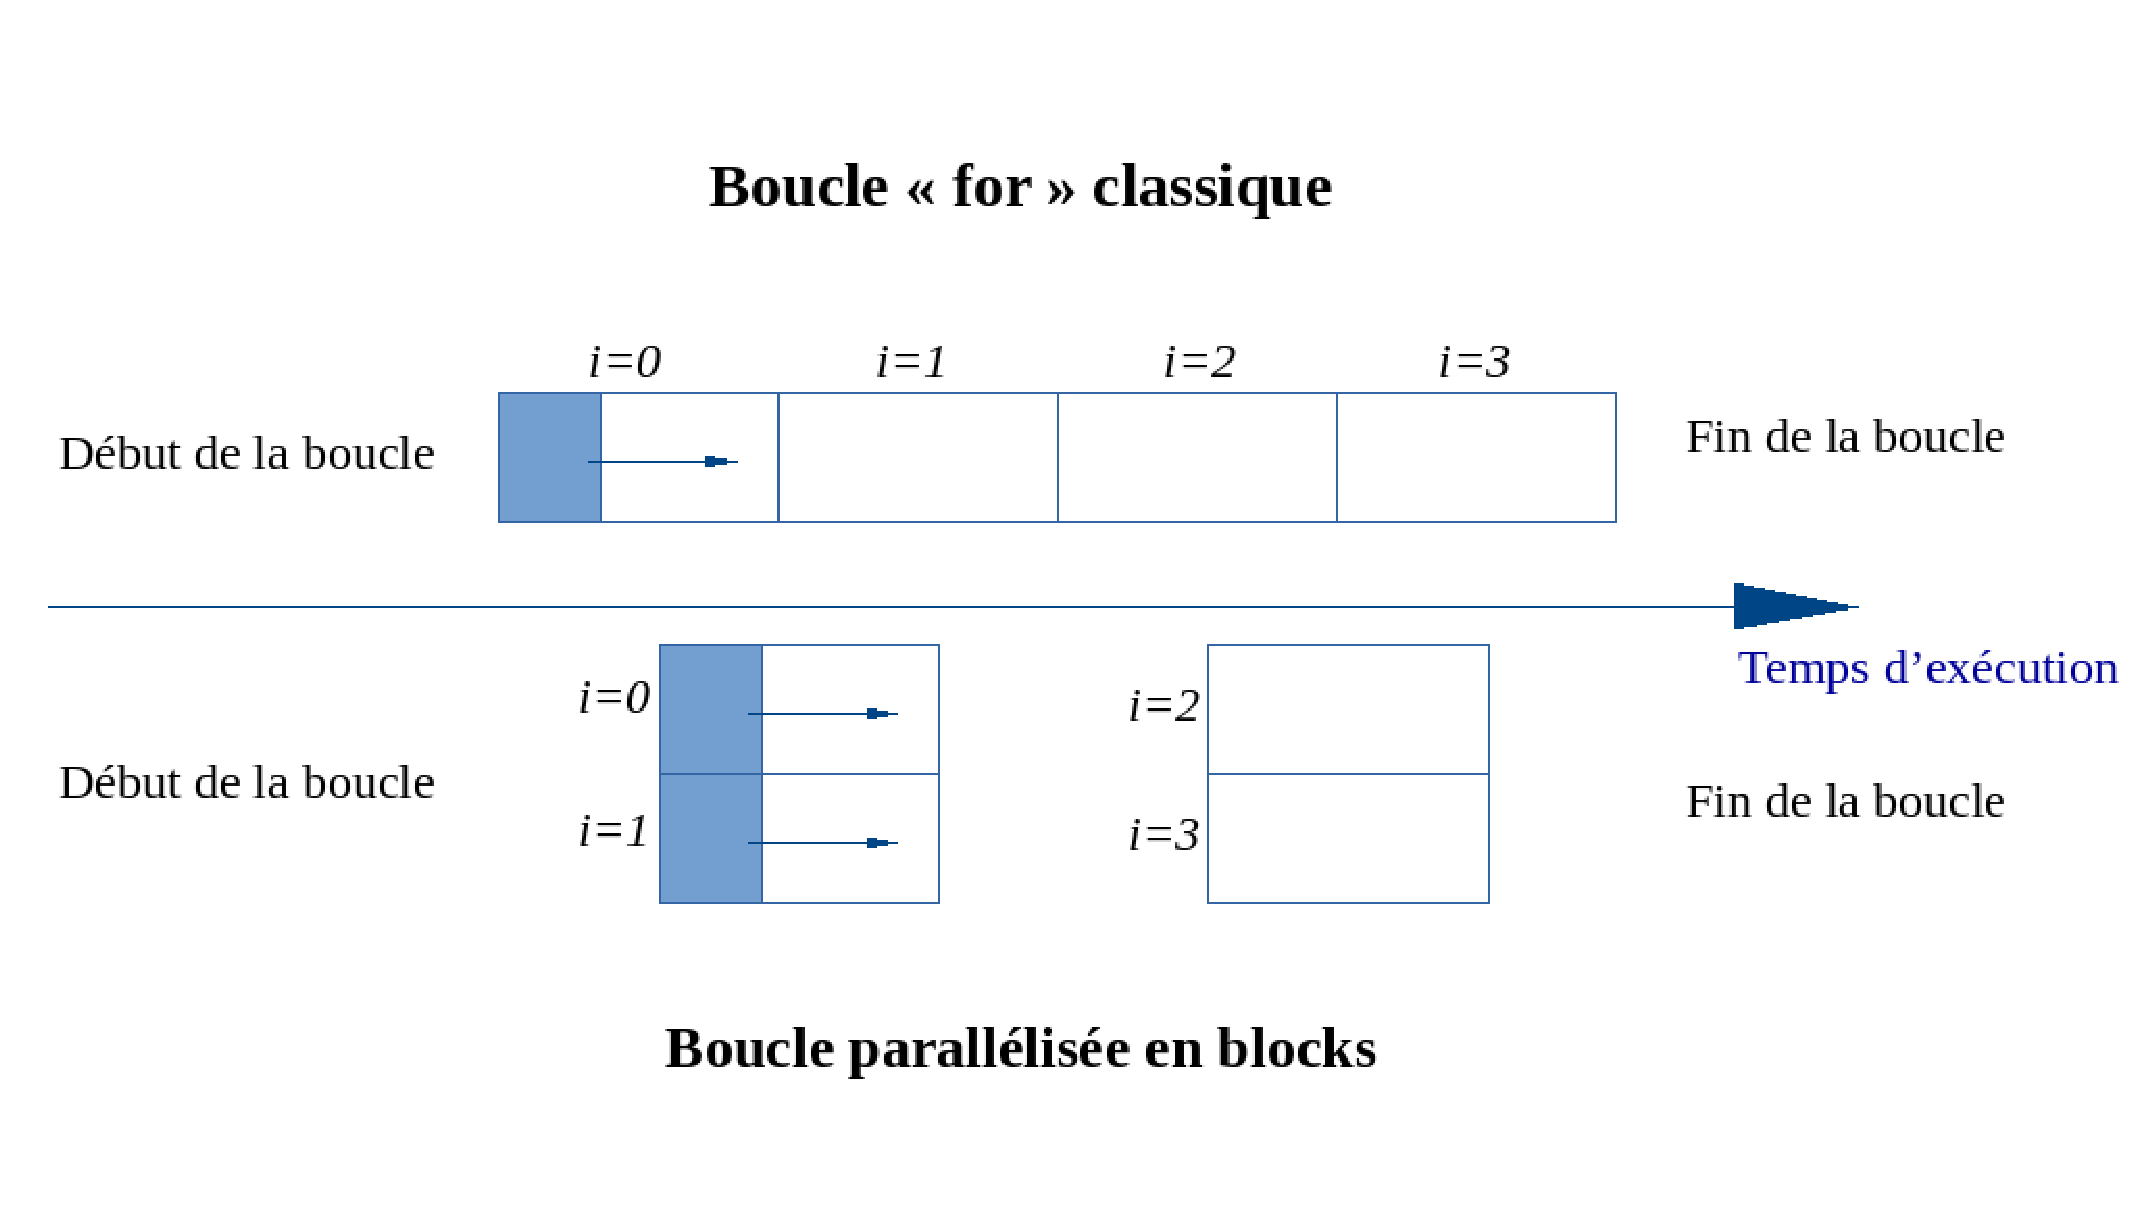
\includegraphics[width=10cm]{Reports/figures/gfor.eps}
		\end{center}	
		\caption{Fonctionnement d'une boucle en parallèle}
		\label{Fonctionnement d'une boucle en parallèle}
	\end{figure}
	
Résultats de MIRTK pour transform-image:
	\begin{figure}[h!]
		\begin{center}
			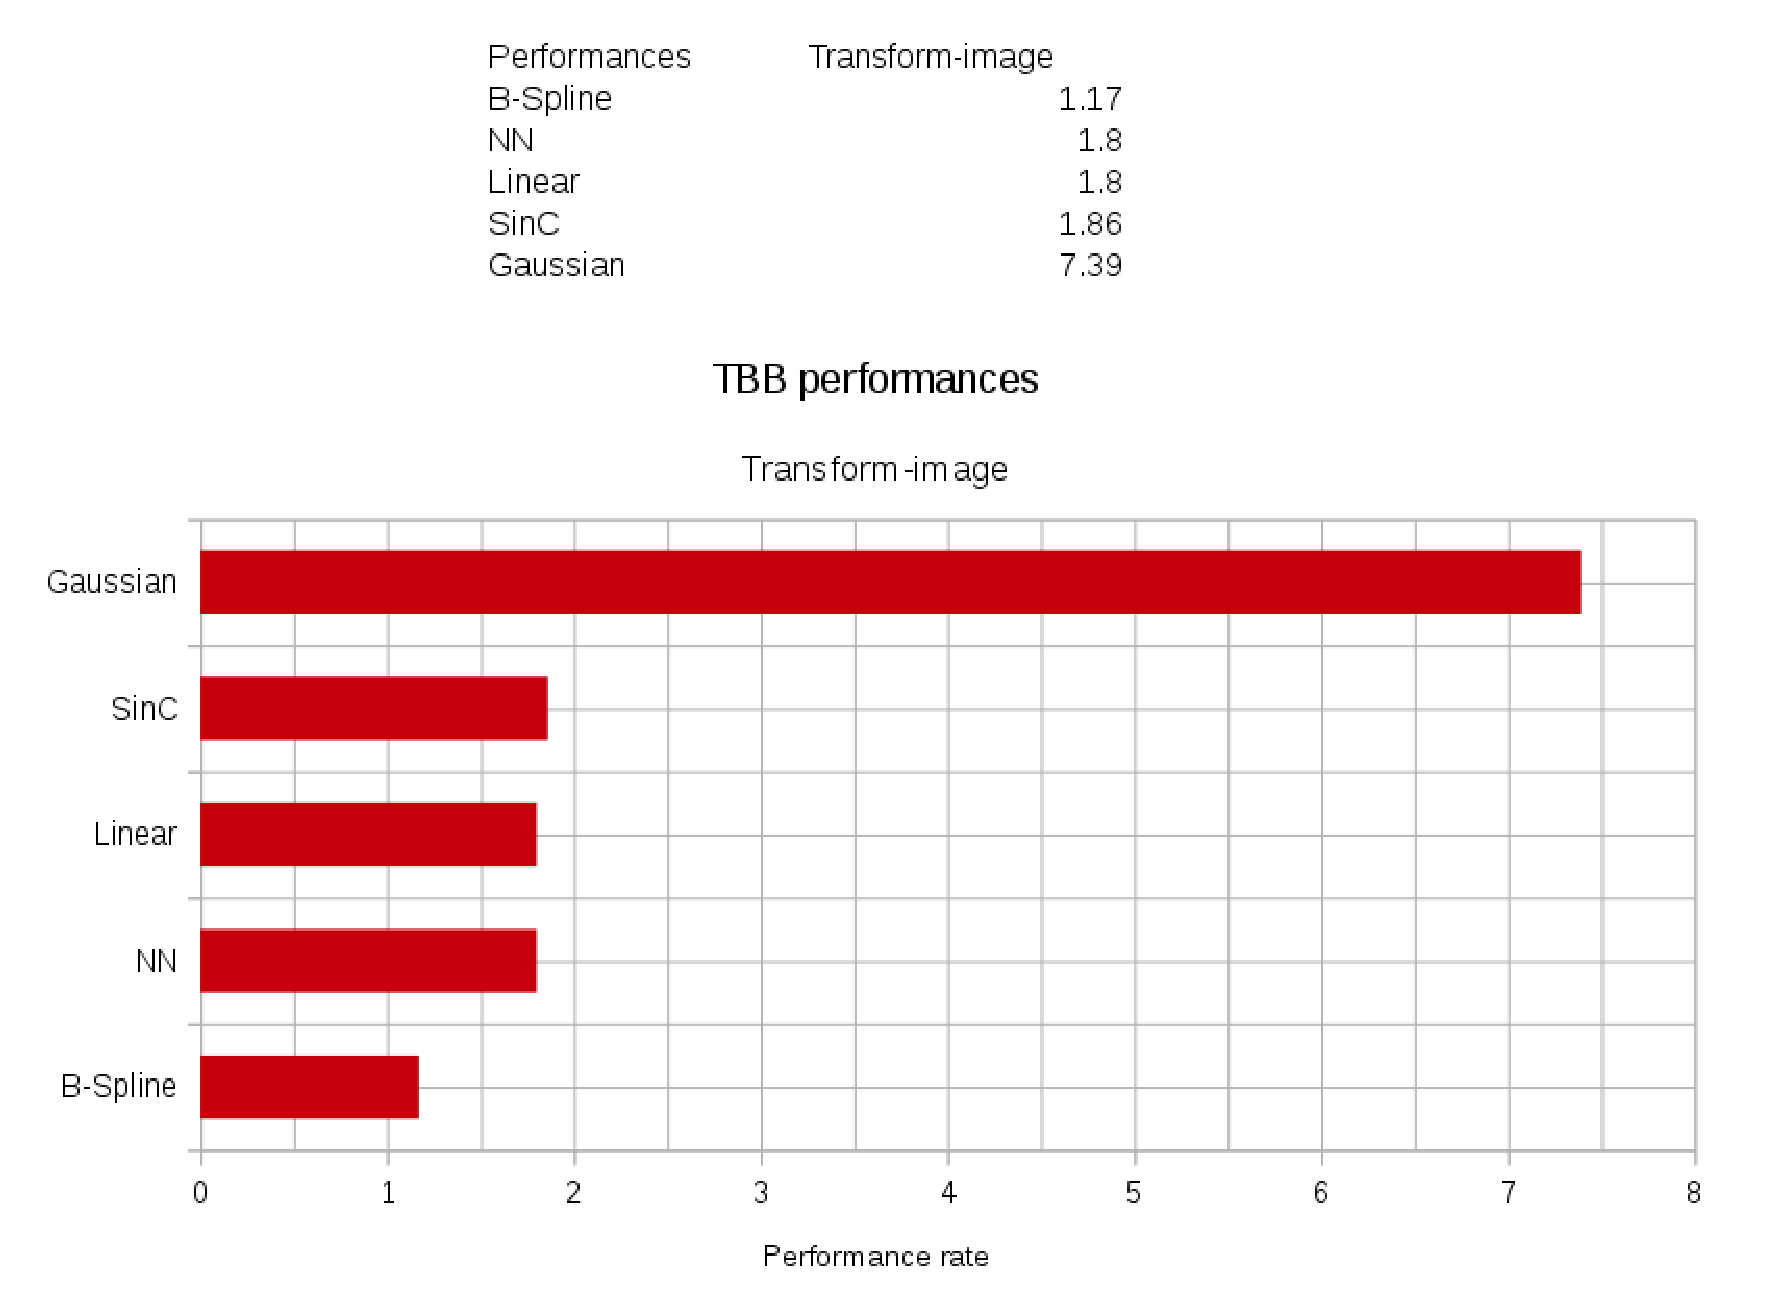
\includegraphics[width=12cm]{Reports/figures/performances_tbb_transform_image.eps}
		\end{center}	
		\caption{Améliorations apportées par TBB pour transform-image}
		\label{Améliorations apportées par TBB pour transform-image}
	\end{figure}
	
%	\newline
%	Le contenus des sous-parties, ainsi que d'éventuelles d'autres sous-parties dépendront du résultat du profilage.
	\subsection{Switch automatique de back-end}
%	Commandes prépocesseur pour indiquer au logiciel quel est le back-end à utiliser (ArrayFire ou Eigen) en fonction de l'opération souhaitée.

	\section{Benchmarking}
	(partie dépendante du déroulement du projet)\newline
	- Analyse des performances obtenues \newline
	- Comparaison avec le profilage initial ? \newline
	- Points où il y a eu des concessions (exemple: alourdir le code pour parvenir à un résultat précis)
	
\chapter{Améliorations et perspectives}
	\section{Au niveau technique...}
	\section{...mais pas seulement!}

\chapter*{Conclusion} % dans cet ordre
\addcontentsline{toc}{chapter}{Conclusion}
\chapter*{Sources}
\addcontentsline{toc}{chapter}{Sources}
https://biomedia.doc.ic.ac.uk/  : image page de garde, partie du texte 1.1.2 \\
http://www.imperial.ac.uk : partie du texte 1.1.1
\chapter*{Table des illustrations}
\addcontentsline{toc}{chapter}{Table des illustrations}
\chapter*{Glossaire}
\addcontentsline{toc}{chapter}{Glossaire}
back-end, front-end, MIRTK, ArrayFire, profilage, run-time, fuite de cache, benchmark
\chapter*{Annexes}
\addcontentsline{toc}{chapter}{Annexes}
\end{document}
